\Chapter{SOAR-based multi-agent system description}\label{chapter:chapter1}

The SOAR cognitive architecture is based on the three stage processing model.
The model consists of the following stages:

\begin{itemize}
    \item Perceive: Accept sensor information from the game
    \item Think: Select and execute relevant knowledge
    \item Act: Execute actions in the game
\end{itemize}

This cycle combined with the SOAR architecture allows for creation of a versatile agent capable of processing and propagating plot events in the game.
The first step allows the agent to modify the state of the working memory.
It can detect visible objects, including other agents and interactables such as containers, doors or even writings.
The second step is divided into two sub-steps, the first executes inference rules and modifies the state of the working memory while the other part executes behavior rules which propose operators.
Operators modify the state of the world, for example by moving the agent, taking the contents of a container, opening doors or interacting with another agent.
This constitutes the last step of the cycle and allows the agent to go back to the first step and update its working memory in preparation for the next step.

This architecture is versatile in that it can be used to model even very complex behaviors.
In order to avoid conflicts in the proposed operators by production rules that try to solve different goals, a goal token can be inserted into the working memory and used as a dependency in the production rules.
This way an agent may have a rule that changes the goal of the agent and thus modifies its next sequence of actions.
The general model of an agent can be seen on figure \ref{fig:agent.drawio.png}.

\begin{figure}[H]
    \centering
    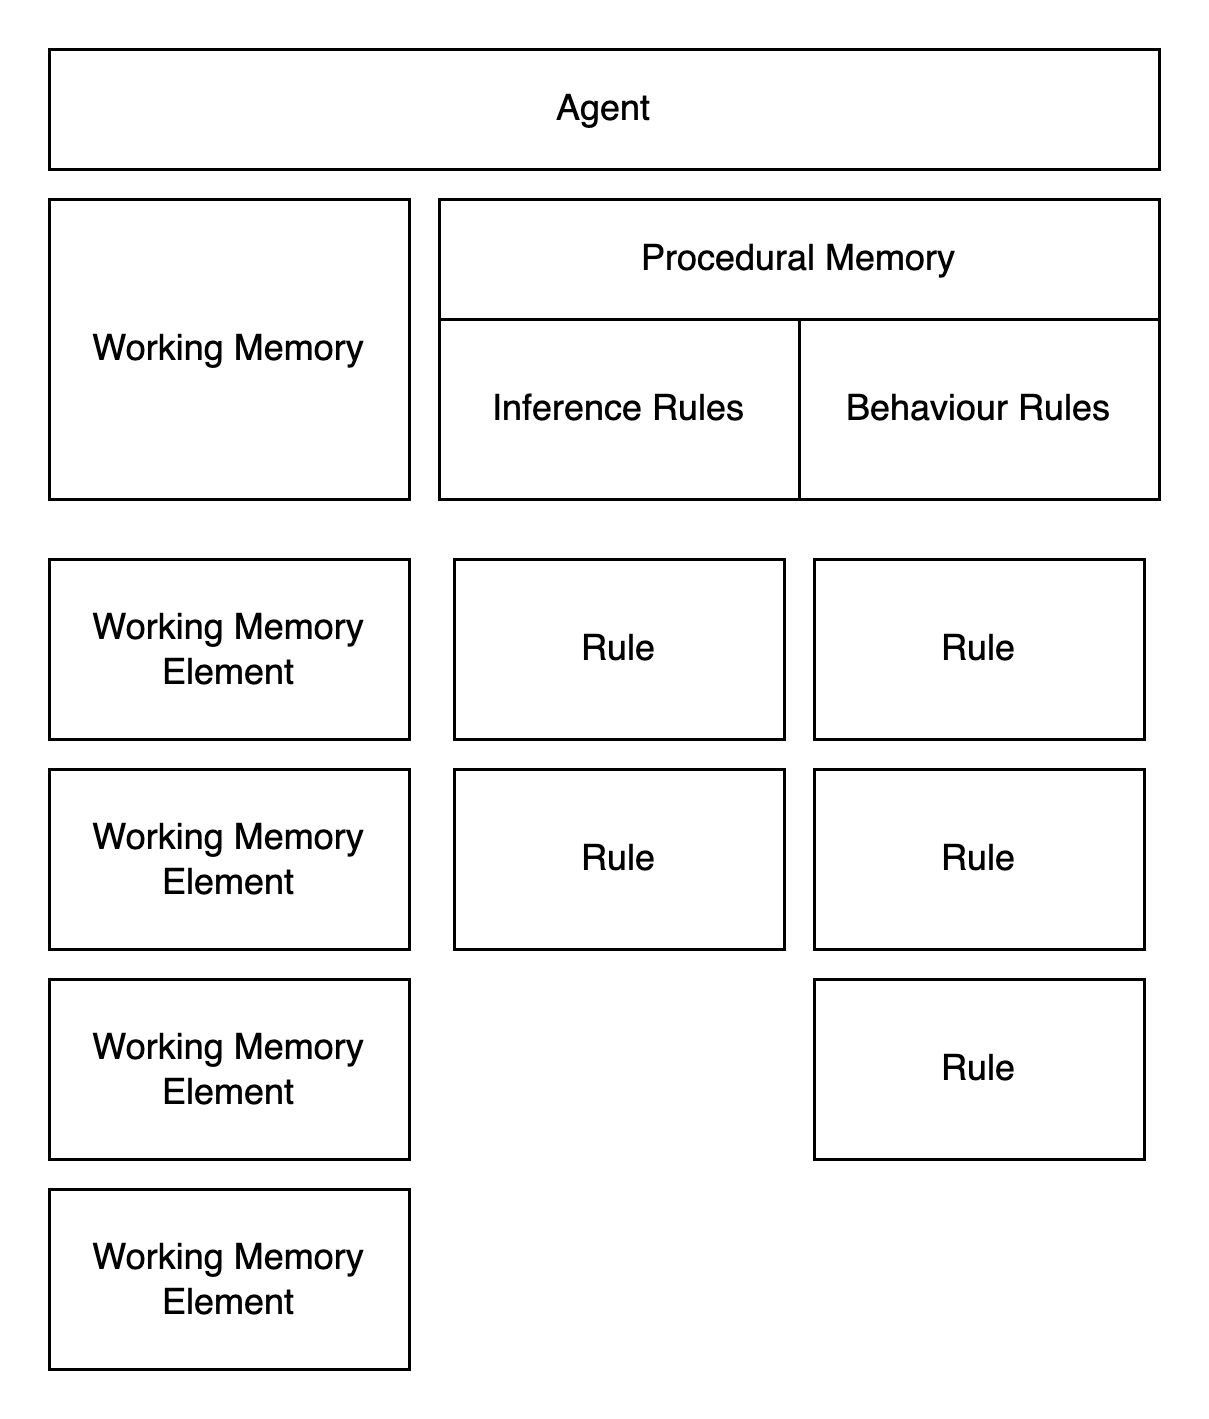
\includegraphics[width=0.6\textwidth]{images/chapter1/agent.drawio.png}
    \caption{Conceptual model of an agent}\label{fig:agent.drawio.png}
\end{figure}

\section{Perceive}

The agent is equipped with simulated sensors that feed into its working memory.
These sensors interact with the simulated world and process the description of the world producing information that is then stored in the working memory of the agent.
Sensory information might include sight, hearing, sense of smell and other commonly thought of senses as well as abstract and arbitrary information that the agent can somehow perceive.
The combined information from all the sensors might produce information regarding the agent's awareness of the vicinity and the location of other agents in the simulated system as well as the state of the agent's body and own position in the game world.
The information is presented to the agent and it is up to the agent to decide what to do with it.
Sensors may only influence working memory of the agent.

All working memory elements produced as a result of perception of the world override the state of the working memory.
This process is called memory unification and usually results in loss of previously stored memories.
Humans in real life do not forget where they have recently been just because they walk.
To facilitate this another mechanism is needed to keep track of the old values from the overridden working memory elements.
Not every working memory element is useful to keep historic values of, however and for the sake of practicality and performance, it is up to the author to choose which values are necessary to maintain a track record of.
Depending on implementation it might make sense to create an inference rule that will save the state of some working memory elements with a prefix to be able to calculate change between the current state of the agent and its previous value.
It is up to the exact implementation to decide how and what is fed to the agent during the perception phase.

Agent's senses might be limited by factors such as weather, terrain, light level, fog, noise and similar.
This means that the information stored in the working memory is not a direct representation of the state of the game world and instead should be treated as interpretation of it done by the agent.
Rules that take into account the state of working memory should always assume that the proposed operator might fail and should use that information to influence the state of the agent's memory.
A blind agent might map out the terrain by virtue of trying to walk into walls repeatedly and keeping track of its own position (under the assumption that they are not moved externally).
This mechanism demonstrates perception feedback and shows that the agent's learning mechanisms can also be implemented by carefully crafting a set of behavior rules.

\section{Think}

Agents have procedural memory that is represented by a collection of production rules that are executed in parallel or sequentially but without respect or guarantees to the exact execution order.
The production rules can be further classified as either inference rules or behavior rules.
Because the rules reside within and form part of the procedural memory, they can be referred to as memory elements.
Irrespective of their type, all production rules influence the working memory of the agent.

Inference rules mutate the state of the working memory but do not propose operators.
They exist for the sake of providing the agent's ability to process and organize their knowledge before attempting to take action.
Because the execution order of the production rules is undefined, it is essential that the designer of the agent ensures no conflicting inference rules are present.
Otherwise undefined behavior might occur, usually causing a rule to override the effects of another rule.

Behavior rules do not modify the state of the working memory but instead produce operators that are used to evaluate the action the agent wishes to perform.
The first restriction is necessary because the system might reject the proposed operators from the executed production rule and thus cause the agent to transition into an inconsistent state.
The operators proposed by each rule are evaluated in an undefined order and when the system accepts the first operator, the rest are not evaluated further.

Each rule might take as input an arbitrary set of working memory elements (WME), check arbitrary preconditions, and in case of behavior rules, produce arbitrary operators that when evaluated will change the state of the simulated world.
Both behavior and inference rules can be simple as well as arbitrarily complex.
A rule can be reactive if its execution depends on the result of the previous execution's evaluation result.

While working memory is perfect for storing the immediate description of the agent's state, it is perhaps ill suited for storage of event based information elements.
For this reason the notion of long-term memory is used for storage of facts characterized by timestamp of occurrence and description of the event.
Procedural memory and production rules therein may also utilize this storage to work with temporal data, for example to facilitate the agent remembering its travel trajectory or recording events such as successful executions of certain actions.
Procedural memory is usually immutable after creation of the agent but it is possible to store a production rule inside of working memory and, by means of another production rule, modify the procedural memory adding the new rule to the bank of rules the agent possesses.
This can simulate agent learning new inference rules and behaviors, for example through reading a book or being taught by other agent.

In general, procedural memory stores the inferences and behaviors of the agent.
Working memory stores the immediate state of the world as known and perceived by the agent.
Long-term memory should be used to store memory elements that are either seldom changing or represent a specific snapshot of time, such as the attitude towards another agent or all the times when the agent was attacked.

\section{Act}

Simulated agents perform actions by choosing and proposing one or more operators that when evaluated express the action's effects.
An operator represents an action that an agent wishes to perform.

The game world is in charge of evaluating the results of the operator and rejecting it in case the agent is not allowed to perform it due to any condition that the agent itself is not aware of.
Because production rules are executed in parallel and thus output multiple operators, it is possible for conflicts to occur.
A single agent may think to move forward and back at the same time.

Because the order in which actions are performed may impact the result, it is important to define a conflict resolution strategy, either for each agent or for the whole game in general.
Such a strategy does not need to necessarily be deterministic as usually it is impossible to determine which operator should take precedence and defining conflict resolution policies for each possible set of conflicting operators is often not a viable approach.

One example of a conflict resolution strategy is a strategy that chooses a random order for conflicting operators and executes them until one is accepted.
This shows the second part of the problem which is conflict detection.
Any two operators can be conflicting in terms of resulting state of the game world.
The simplest approach is not allowing the agent to execute multiple operators at the same time and instead force it to choose one specific action instead.

Another more complex idea is to introduce the concept of operator's utility score.
The idea comes from utility based AI, a common technique for modeling agent's behavior without introducing a cognitive architecture \cite{dill2012design}.
This strategy would require the ability to estimate the utility of each operator and choose to order all proposed operators by the utility score.
The score could be calculated either based on the projection of the operator's effect or through retrospection of previous execution.
The second approach should also be supplemented with context of the previous execution to prevent situations where the agent will fail to attack another agent because that agent is too far away and thus calculate that the attack operator does not do anything and thus provide zero utility.

Providing the context of execution for the operator and comparing it to the current context provides yet another challenge of being able to express the difference in situation in a deterministic way to determine if the utility of the previous situation should influence the utility of the current proposition.
Because of the complexity of this approach exceeding the scope of this thesis, for the sake of experiments a simple random choice strategy was chosen for conflict resolution.

\section{Desired system behavior}

Because the multi-agent system described in this thesis needs to be able to simulate propagation of information in a virtual population of simulated game characters (represented by individual agents), the system needs to be able to express the possible interactions between agents.
For the sake of modeling information propagation, an epidemiological model was chosen.
For this reason the list of possible agent interactions is constrained to the following list:

\begin{itemize}
    \item infect
    \item walk
\end{itemize}

The system should be able to represent an agent possessing limited field of vision expressed by the maximum sight distance under which it becomes aware of other agents.
The state of infection of another agent should also be available to the agent when it is able to visually perceive the other agent.

An example scenario could start with an agent initialized at some randomly chosen coordinates.
During the first stage of simulation, the agent will see other adjacent agents within its sight distance.
For the sake of illustration, let them be labeled as $A_1$, $A_2$ and $A_3$.
The agent is not infected and thus proposes random direction walk operators causing it to roam.
$A_1$ is infected and reaches the agent, infecting it.
Then, because agent now has the rule governing its behavior under infection, it remembers the position of all the previously seen agents and wishes to infect them.
It knows that $A_1$ is already infected.
The agent does not see agent $A_2$ anymore but can still see agent $A_3$.
It walks towards the position of agent $A_3$ and infects it.
It still does not see agent $A_2$ but remembers that its last known position.
It walks towards it and eventually notices agent $A_2$ which means it now knows it updated location and changes direction to head towards it.
After infecting the second agent, it is left with no more susceptible agents that it knows the position of and thus roams around randomly again.

It should be worth noting that at each moment the infected agent should be proposing the $Infect$ operator which during evaluation will be rejected if there are no adjacent agents to infect.
This means that the behavior rule does not need to take into account the actual position of the other agents to try and infect them.

Because this operator will be rejected, another operator proposed by the same rule will be evaluated.
In this example the second operator would be the $Walk$ operator with the direction that the agent should head during the particular simulation step.

This shows that the agent is capable of accumulating experience during its lifetime and thus react to both the state of the simulation it is perceiving at any given moment but also to information it retained.
It shows also the memory elements of the agent are not lost when they are not continuously provided at each simulation step, meaning that the agent does not forget the last seen position of each agent even if it stopped being able to see them anymore.

\section{Conclusions}

The chosen cognitive architecture and described solution should allow for implementation of an epidemiological model.
In order to evaluate the approach chosen in this thesis, the results of the simulation will be compared with a mathematical model directly.
The first of the research questions proposed in the thesis objective can be answered based on the analysis of the cognitive architectures described previously.
The SOAR cognitive architecture (and others similar to it) can be used for a multi-agent system to implement information propagation in games based on a collection of production rules defining the agents' behaviors.
